\documentclass[11pt]{beamer}
\usetheme{Frankfurt}
\usecolortheme{lily}
\usepackage[utf8]{inputenc}
\usepackage[english]{babel}
\usepackage{amsmath}
\usepackage{amsfonts}
\usepackage{amssymb}
\usepackage{graphicx}
\usepackage{tabularx}
%\usepackage{circuitikz}
\author{Maximilian Heim}
\title{Hardware Trojan Detection}
%\setbeamercovered{transparent} 
%\setbeamertemplate{navigation symbols}{} 
\logo{
\includegraphics[width=1.5cm]{1200px-Hsas_logo.svg.png}}
\institute{University Albstadt-Sigmaringen} 
\date{\today} 
\subject{Hardware Cyber-Security}
\begin{document}

\begin{frame}
\titlepage
\end{frame}

\begin{frame}
\tableofcontents
\end{frame}

\section{Introduction}
\subsection{Hardware Trojans}
\begin{frame}
    \frametitle{Was sind Hardware Trojaner?}
    \begin{itemize}
    \item Bösartige Modifikation eines Integrierten Schaltkreises
    \item Trigger (Time bombs, cominational...)
    \item Payload (Denial of service, keys\ldots)
    \end{itemize}
    \begin{figure}
        \caption{Theoretischer Aufbau eines HW Trojaners}
        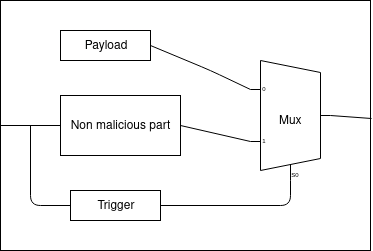
\includegraphics[width=0.5\textwidth]{triggerpayload.png}
        \label{trpl}
    \end{figure}
\end{frame}

\section{Destruktive Detektion}
\begin{frame}
    \frametitle{Destruktives Reverse Engineering}
    \begin{itemize}
        \item Entfernen der Oberfläche
        \item Visuelle Inspektion
        \item Vergleich mit Golden Sample
        \item Vorteile: 
        \begin{enumerate}
            \item 100 \% Erkennungsrate
        \end{enumerate}
        \item Nachteile:
        \begin{enumerate}
            \item Testet nur einen Chip
            \item Destruktiv
            \item Zeitaufwändig
        \end{enumerate}
        \item Jedoch: Sinnvoll in Kombination mit anderen Verfahren
    \end{itemize}
\end{frame}
\section{Nicht-Destruktive Detektion}
\begin{frame}
    \frametitle{Funktionstests}
    \begin{itemize}
        \item Beobachten der Ausgabe bei bestimmten Eingängen
        \item Vergleich mit Golden Sample
        \item Problem: Großer Trojan Space
        \item Vorteile:
        \begin{enumerate}
            \item Sehr einfacher Testaufbau
            \item Bei bekannten Testvektoren $\rightarrow$ 100 \% Erkennungsrate
            \item Hunderte IC's können parallel getestet werden
        \end{enumerate}
        \item Nachteile:
        \begin{enumerate}
            \item Je nach Komplexität des IC's sehr zeitaufwändig/unmöglich
        \end{enumerate}
    \end{itemize}
\end{frame}
\begin{frame}
    \frametitle{Funktionstests: Statistischer Ansatz}
    \begin{itemize}
        \item R.S. Chakraborty et al, "MERO: A Statistical Approach for Hardware Trojan Detection"
        \item \url{https://link.springer.com/content/pdf/10.1007/978-3-642-04138-9_28.pdf}
        \item Netzliste $\rightarrow$ Testvektoren
        \item Vektoren werden N mal getestet (Kombinatorisch-sequentielle HW Trojaner)
        \item Reduktion der Testzeit um 85 \%
    \end{itemize}
\end{frame}

\begin{frame}
    \frametitle{Seitenkanaltest}
    \begin{itemize}
        \item Beobachten der Leistungsaufnahme/Pfadverzögerung \item Vergleich mit Golden Sample
        \item Vorteile:
        \begin{enumerate}
            \item Erkennung ohne Aktivierung
            \item Sehr einfacher Testaufbau
            \item Hohe Erkennungsrate
            \item Hunderte IC's können parallel getestet werden
        \end{enumerate}
        \item Nachteile:
        \begin{enumerate}
            \item Produktionsvariationen
            \item Bei sehr kleinen Trojanern kann die Leakage sehr klein werden
        \end{enumerate}
    \end{itemize}
\end{frame}
\begin{frame}
    \frametitle{Seitenkanaltest: Fingerprinting}
    \begin{itemize}
        \item D. Agrawal et al, "Trojan Detection using IC Fingerprinting"
        \item \url{https://ieeexplore.ieee.org/stamp/stamp.jsp?tp=&arnumber=4223234}
        \begin{enumerate}
            \item Auswahl zufälliger Schaltkreise
            \item Aufnahme von Power Traces
            \item Fingerprint erzeugen
            \item Destruktives Reverse Engineering der Chips
            \item Vergleiche Fingerprints von zu testenden Chips mit Referenz
        \end{enumerate}
    \end{itemize}
\end{frame}

\section{Fazit}
\begin{frame}
    \frametitle{Fazit}
    \begin{itemize}
        \item Destruktive Detektion ungeeignet für Testen von ICs die verwendet werden sollen
        \item Gegenüberstellung von Funktionstests und Seitenkanaltests:
    \end{itemize}
    \begin{tabular}{|m{1cm}|m{4.2cm}|m{4.2cm}|}
        \hline
         & Funktionstests & Seitenkanaltests \\
        \hline
        Pros & 1. Effektiv für kleine Trojaner \newline 2.Produktionstoleranz unabhängig & 1.Effektiv für große Trojaner \newline 2. einfache Testerzeugung \\
        \hline
        Cons & 1. Testerzeugung komplex & 1. Anfällig für Produktionstoleranzen \newline 2. Detektion von kleinen Trojanern schwierig\\
        \hline
    \end{tabular}
    \begin{itemize}
        \item Wie man sieht: Die Verfahren ergänzen sich $\rightarrow$ Kombination beider Verfahren
    \end{itemize}
\end{frame}
\section*{Quellen}
\begin{frame}
    \frametitle{Quellen}
    \begin{itemize}
    \item \url{https:/d/dl.acm.org/doi/pdf/10.1145/2906147}
    \item \url{https://ieeexplore.ieee.org/stamp/stamp.jsp?tp=&arnumber=5340158}
    \item \url{https://www.fkie.fraunhofer.de/content/dam/fkie/de/documents/HWT-Bericht/HWT-Bericht_Cover.pdf}
    \item \url{https://en.wikipedia.org/wiki/Hardware_Trojan} 
\end{itemize}
\end{frame}

\end{document}